\documentclass[t,mathserif,10pt,aspectratio=1610]{beamer}
% option "t" means align top
% option "handout" for handout mode (each frame takes only one page)
% option "notes" to add notes pages

\setbeamertemplate{footline}[frame number]

\mode<presentation>
{
  \usetheme{bo}
}

\newcommand{\mycite}[1]{{\footnotesize [\textit{#1}]}}

\newcommand{\centergraphics}[2]{
  \begin{center}
  \includegraphics[width=#1\textwidth]{#2}
  \end{center}} % end newcommand

\newcommand{\centerboxgraphics}[2]{
  \begin{center}
  \fbox{\includegraphics[width=#1\textwidth]{#2}}
  \end{center}} % end newcommand

\newcommand\blfootnote[1]{%
  \begingroup
  \renewcommand\thefootnote{}\footnote{#1}%
  \addtocounter{footnote}{-1}%
  \endgroup
}


\newtheorem{myfact}{Fact}
\newtheorem{prop}{Proposition}
\newtheorem*{theorem*}{Theorem}
\newtheorem{question}{Question}

\DeclareMathOperator*{\E}{\mathbb{E}}


\newcommand{\kl}{\textnormal{KL}}
\newcommand{\relint}{\textnormal{relint}}
\newcommand{\tr}{\top}
\newcommand{\id}{\mathop{\mathrm{id}}}
\newcommand{\Var}{\mathop{\mathrm{Var}}}

\newcommand{\loss}{\ell}

\newcommand{\A}{\mathcal{A}}
\newcommand{\B}{\mathcal{B}}
\newcommand{\D}{\mathcal{D}}
\newcommand{\F}{\mathcal{F}}
\newcommand{\G}{\mathcal{G}}
\renewcommand{\H}{\mathcal{H}}
\newcommand{\I}{\mathcal{I}}
\newcommand{\K}{\mathcal{K}}
\renewcommand{\L}{\mathcal{L}}
\newcommand{\M}{\mathrm{M}}
\newcommand{\N}{\mathbb{N}}
\renewcommand{\O}{\mathcal{O}}
\renewcommand{\P}{\mathcal{P}}
\newcommand{\Q}{\mathcal{Q}}
\newcommand{\R}{\mathcal{R}}
\let\oldS\S % section symbol!
\newcommand{\sect}{\mbox{\oldS\hspace{-.1mm}}}
\renewcommand{\S}{\mathcal{S}}
\newcommand{\T}{\mathcal{T}}
\newcommand{\V}{\mathcal{V}}
\newcommand{\W}{\mathcal{W}}
\newcommand{\Y}{\mathcal{Y}}
\newcommand{\X}{\mathcal{X}}

\renewcommand{\vec}[1]{{\mathbf{#1}}}
\newcommand{\1}{\vec{1}}
\newcommand{\0}{\vec{0}}
\renewcommand{\b}{\vec{b}}
\newcommand{\e}{\vec{e}}
\newcommand{\g}{\vec{g}}
\renewcommand{\l}{\boldsymbol{\ell}}
\newcommand{\m}{\vec{m}}
\renewcommand{\o}{\mathit{o}}
\newcommand{\p}{\vec{p}}
\newcommand{\q}{\vec{q}}
\renewcommand{\r}{\vec{r}}
\newcommand{\s}{\vec{s}}
\renewcommand{\u}{\vec{u}}
\renewcommand{\v}{\vec{v}}
\newcommand{\w}{\vec{w}}
\newcommand{\x}{\vec{x}}
\newcommand{\y}{\vec{y}}
\newcommand{\z}{\vec{z}}

\newcommand{\convhull}{\mathsf{Conv}}
\newcommand{\conv}{\convhull}
\newcommand{\ext}{\mathrm{ext}}
\newcommand{\clo}{\mathrm{cl}}
\newcommand{\linear}{\mathsf{Lin}}
\newcommand{\affine}{\mathsf{Aff}}
\newcommand{\subgrad}[1]{d #1}
\newcommand{\subtang}[1]{d #1}
\newcommand{\subdiff}[1]{\partial #1}
\newcommand{\selsubgrad}[2]{\in \partial {#1}}%|_{#2}}
\newcommand{\toto}{\rightrightarrows}
\newcommand{\eval}{\mathsf{Eval}}
\newcommand{\nondiff}{\mathsf{nondiff}}
\newcommand{\cell}{\mathrm{cell}}
\newcommand{\lsc}{l.s.c.}
\newcommand{\dom}{\mathrm{dom}}
\newcommand{\defeq}{\doteq}%\vcentcolon=} % define equals
\newcommand{\ones}{\mathbf{1}}
\newcommand{\abs}[1]{\left\lvert #1 \right\rvert}
\newcommand{\sgn}{\mathrm{sgn}}
\newcommand{\im}{\mathop{\mathrm{im}}}
\newcommand{\spn}{\mathop{\mathrm{span}}}
\newcommand{\affspn}{\mathop{\mathrm{affinespan}}}

\newcommand{\elic}{\mathsf{elic}}
\newcommand{\elici}{\elic_\ID}
\newcommand{\iden}{\mathsf{iden}}
\newcommand{\EL}{\mathcal{E}}
\newcommand{\ID}{\mathcal{I}}
\newcommand{\ES}{\mathrm{ES}}
\newcommand{\lbar}{\underline{L}}

\def\reals{\mathbb{R}}
\def\integers{\mathbb{Z}}
\def\extreals{\mathbb{\overline{R}}}

\newcommand{\argmin}{\mathop{\mathrm{argmin}}}
\newcommand{\argmax}{\mathop{\mathrm{argmax}}}
\newcommand{\arginf}{\mathop{\mathrm{arginf}}}
\newcommand{\argsup}{\mathop{\mathrm{argsup}}}





\usepackage{adjustbox}


\title{\Large\textbf{Information Elicitation \\ and Design of Surrogate Losses}}
\titlegraphic{
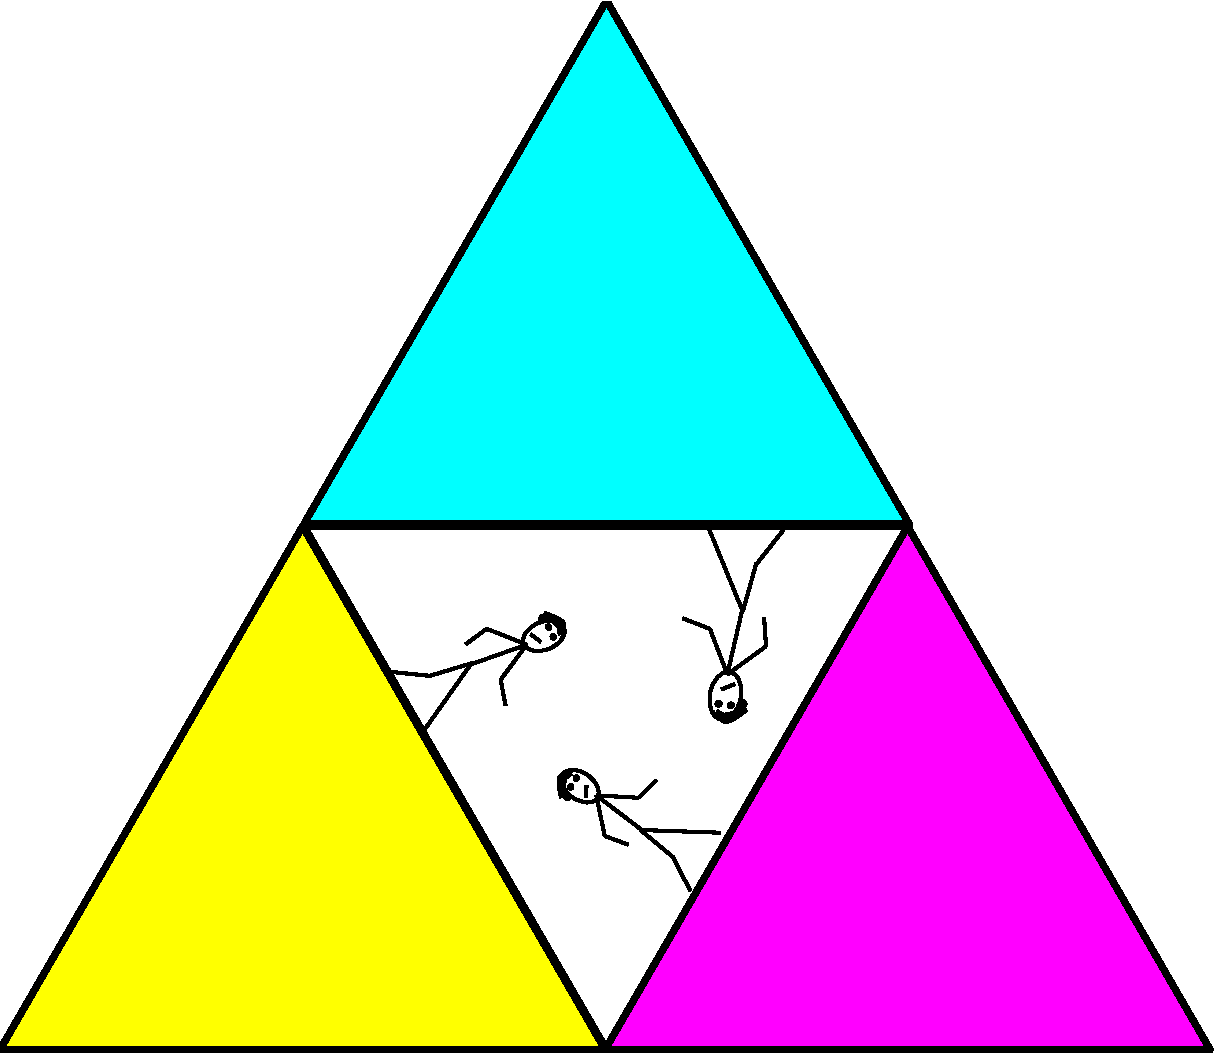
\includegraphics[width=.35\textheight]{figs/logo}
}

\author[Bo Waggoner]{{\textbf{Bo Waggoner}} \and \textbf{University of Colorado, Boulder}}
\date{\textbf{Peking University \\ October 30, 2020}}

\begin{document}

%%%%%%%%%%%%%%%%%%%%%%%%%%%%%%%%%%%%%%%%%%%%%%%%%%%%%%%%%%%%%%%
\begin{frame}
  \titlepage

  {\footnotesize Based on joint work with Jessie Finocchiaro and Rafael Frongillo (U. Colorado, Boulder).}
\end{frame}

%%%%%%%%%%%%%%%%%%%%%%%%%%%%%%%%%%%%%%%%%%%%%%%%%%%%%%%%%%%%%%
\begin{frame}{Motivation 1: Design of surrogate loss functions}{}
\begin{itemize}[<+->]
  \item We measure how well an algorithm predicts using a loss function.  \\
  \item Often, natural or popular losses are \myem{intractable.}  \\
  \item So, we minimize another one -- the \blueem{surrogate}.  \\
\end{itemize}

\pause
\vskip1em
\centergraphics{0.9}{figs/hinge}
\end{frame}

%%%%%%%%%%%%%%%%%%%%%%%%%%%%%%%%%%%%%%%%%%%%%%%%%%%%%%%%%%%%%%
\begin{frame}{Key tool and motivation 2: Information elicitation}{}
\begin{itemize}[<+->]
  \item A forecaster is asked to make a prediction about a future event.  \\
  \item She is assigned a \myem{loss} based on the outcome.  \\
  \item She minimizes expected loss.
\end{itemize}

\pause
\vskip1em
\centergraphics{0.9}{figs/forecast}
\end{frame}

%%%%%%%%%%%%%%%%%%%%%%%%%%%%%%%%%%%%%%%%%%%%%%%%%%%%%%%%%%%%%%
\begin{frame}{Connection between problems}{}
\vskip6em
{\large
  \[ \argmin_{r \in \R} \E_{Y\sim p} \ell(r, Y)   \]
} % end large
\end{frame}

%%%%%%%%%%%%%%%%%%%%%%%%%%%%%%%%%%%%%%%%%%%%%%%%%%%%%%%%%%%%%%
\begin{frame}{Outline}{}
\vskip2em
\begin{enumerate}
  \item Concepts and definitions from information elicitation  \\
        \hint{what do you get when you minimize a loss?}
  \vskip1em
  \item Surrogate loss functions for machine learning
  \vskip1em
  \item The embedding approach; our contributions
\end{enumerate}
\end{frame}

%%%%%%%%%%%%%%%%%%%%%%%%%%%%%%%%%%%%%%%%%%%%%%%%%%%%%%%%%%%%%%
\begin{frame}{}{}
  \vskip12em
  {\large \textbf{Part 1:} Concepts and definitions from information elicitation}
\end{frame}

%%%%%%%%%%%%%%%%%%%%%%%%%%%%%%%%%%%%%%%%%%%%%%%%%%%%%%%%%%%%%%
\begin{frame}{Information elicitation}{}
\blueem{What do you get when you minimize a loss?}
\begin{equation} \label{eqn:elicit}
  \Gamma(p) := \argmin_{r \in \R} \E_{Y\sim p} \ell(r, Y)
\end{equation}

\vskip1em
 
\only<1-7>{
  Examples:
  \begin{itemize}
    \item $\ell(r, y) = (r - y)^2$       \pause \hintright{$\Gamma(p) = \E_{Y\sim p} Y$ ~(mean)}
    \pause \item $\ell(r, y) = |r - y|$  \pause \hintright{median}
    \pause \item $\ell(r, y) = \begin{cases} 0 & r=y \\ 1 & \text{otherwise} \end{cases}$  \pause \hintright{mode}
    \pause \item $\ell(r, y) = ??$       \hintright{variance}
  \end{itemize}
} % end only
\only<8>{
  \begin{itemize}
    \item $\Gamma: \Delta_{\Y} \to 2^{\R}$ is a \blueem{property} of the distribution $p$.
    \item $\Gamma$ is \blueem{elicitable} if there exists $\ell$ such that (\ref{eqn:elicit}) holds.
  \end{itemize}
} % end only
 
\end{frame}

%%%%%%%%%%%%%%%%%%%%%%%%%%%%%%%%%%%%%%%%%%%%%%%%%%%%%%%%%%%%%%
\begin{frame}{Information elicitation - the picture}{}
\only<1>{The simplex $\Delta_{\Y}$ for $\Y = \{10,20,30\}$:}
\only<2->{
  \begin{itemize}
    \item<2-> A property is a partition of the simplex.
    \item<2-> The \blueem{level set} of $r$ is $\{p : \Gamma(p) = r\}$.
  \end{itemize}
} % end only

\vskip0.5em
\only<1>{\centergraphics{0.8}{figs/simplex-1}}
\only<2>{\centergraphics{0.8}{figs/simplex-2}}
\only<3>{\centergraphics{0.8}{figs/simplex-3}}
\end{frame}

%%%%%%%%%%%%%%%%%%%%%%%%%%%%%%%%%%%%%%%%%%%%%%%%%%%%%%%%%%%%%%
\begin{frame}{Key basic fact}{}
\begin{theorem}
  If a property is elicitable, then all of its level sets are convex sets.
\end{theorem}

\vskip0.5em
\only<1>{\centergraphics{0.8}{figs/simplex-3}}
\only<2>{\centergraphics{0.8}{figs/simplex-4}}
\end{frame}

%%%%%%%%%%%%%%%%%%%%%%%%%%%%%%%%%%%%%%%%%%%%%%%%%%%%%%%%%%%%%%
\begin{frame}{Dealing with non-elicitable properties}{}
\blueem{Indirect elicitation:} Elicit some \emph{other} properties, then compute $\Gamma(p)$.

\pause
\vskip1em
\myem{Example:} elicit variance using mean, second moment.

\pause
\vskip1em
 \[ L((\mu_1, \mu_2), y) = (\mu_1 - y)^2 + (\mu_2 - y^2)^2 . \]

\pause
\vskip1em
\blueem{Elicitation complexity\footnote{Frongillo and Kash, 2015.}} of $\Gamma$: fewest parameters needed to indirectly elicit $\Gamma$.  \\
\hint{Variance: 2.}

\end{frame}

%%%%%%%%%%%%%%%%%%%%%%%%%%%%%%%%%%%%%%%%%%%%%%%%%%%%%%%%%%%%%%
\begin{frame}{}{}
  \vskip12em
  {\large \textbf{Part 2:} Surrogate loss functions for machine learning}
\end{frame}

%%%%%%%%%%%%%%%%%%%%%%%%%%%%%%%%%%%%%%%%%%%%%%%%%%%%%%%%%%%%%%
\begin{frame}{Supervised learning setting}{}
\begin{itemize}[<+->]
  \item Space of features $\X$
  \item Space of outcomes $\Y$  \\
        \hint{finite, e.g. labels}
  \item Data point: $(x,y) \in \X \times \Y$.
  \item Hypothesis $h: \X \to \R$.
  \item Target loss $\ell: \R \times \Y \to \reals_{\geq 0}$.
\end{itemize}

\pause
\vskip1em
\blueem{Goal:} for a distribution $\D$ on $\X \times \Y$, \\
find a hypothesis minimizing expected loss:
  \[ \min_h \E_{X,Y \sim \D} \ell( h(x), y) . \]

\pause
\vskip1em
Let $p_x = $ conditional distribution of $Y$ given $X=x$.  \\
\myem{Bayes optimal:} $h(x) = \gamma(p_x)$  \\
\hint{where $\gamma$ is the property elicited by $\ell$.}
\end{frame}

%%%%%%%%%%%%%%%%%%%%%%%%%%%%%%%%%%%%%%%%%%%%%%%%%%%%%%%%%%%%%%
\begin{frame}{Why surrogate losses?}{}
\textbf{Problem 1:} wish to learn $h: x \mapsto \gamma(p_x)$, but $\gamma$ is not elicitable.

\pause
\vskip0.5em
\textbf{Problem 2:} $\ell$ is \myem{intractable.}

\pause
\vskip0.5em
\blueem{Solutions:} use a surrogate loss $L$.

\pause
\vskip1em
\centergraphics{0.6}{figs/logistic}
\end{frame}

%%%%%%%%%%%%%%%%%%%%%%%%%%%%%%%%%%%%%%%%%%%%%%%%%%%%%%%%%%%%%%
\begin{frame}{What makes a surrogate loss good?}{}
(1) tractability, (2) correct relationship to $\ell$.

\pause
\vskip1em
\blueem{(1) Tractability} of a surrogate loss $L: \reals^d \times \Y \to \reals_{\geq 0}$
\begin{itemize}[<+->]
  \item Convex
  \item $d$ is small\footnote{\emph{convex calibration dimension}, Ramaswamy \& Agarwal 2016.}
\end{itemize}

\pause
\vskip1em
\blueem{(2) Relationship} to $\ell$:
\begin{itemize}[<+->]
  \item Note: need combination of $L$ and \blueem{link} $\psi: \reals^d \to \R$.
  \item \textbf{Consistency:} optimizing $L$, then applying $\psi$, leads to optimizing $\ell$.
  \item \textbf{Calibration:} if $\psi(u)$ is suboptimal for $\ell$, then $u$ is suboptimal for $L$ (for each $p_x)$.
  \item \blueem{Our point (new work):} it is necessary and almost sufficient for $L,\psi$ to \blueem{indirectly elicit} $\gamma$.  \\
        \hint{Lower bounds, etc.}
\end{itemize}
\end{frame}

%%%%%%%%%%%%%%%%%%%%%%%%%%%%%%%%%%%%%%%%%%%%%%%%%%%%%%%%%%%%%%
\begin{frame}{}{}
  \vskip12em
  {\large \textbf{Part 3:} The embedding approach; our contributions.}
\end{frame}

%%%%%%%%%%%%%%%%%%%%%%%%%%%%%%%%%%%%%%%%%%%%%%%%%%%%%%%%%%%%%%
\begin{frame}{How do you find a good surrogate?}{}
Suppose $\R$ is finite (e.g. classification, ranking, top-$k$, \dots).

\pause
\vskip1em
One idea: \textbf{embed} $\ell$ as follows:
\begin{itemize}[<+->]
  \item For each $r \in \R$, choose some $u_r \in \reals^d$.  \\
        \hint{embedding points}
  \item Find a convex surrogate $L$ such that $u_r \in \argmin L(\cdot ; p)$ if and only if $r \in \argmin \ell(\cdot ; p)$.
  \item Set $\psi(u_r) = r$ for each $r$.
  \item Choose $\psi(u)$ somehow on the rest of $\reals^d$.
        \hint{$(L,\psi)$ is an embedding of $\ell$}
\end{itemize}

\pause
\vskip1em
\textbf{Problems:} when does such an $L$ exist? how to find it?

\begin{theorem*}
  We can automatically, efficiently construct an embedding $L$ of $\ell$ from $\ell$ using dimensions $d = |\Y|-1$.
\end{theorem*}

\pause
\emph{Proof idea:}
Use the convex conjugate of the Bayes risk of $\ell$.  \\
\hint{Not really a new construction; e.g. prediction markets!}
\end{frame}

%%%%%%%%%%%%%%%%%%%%%%%%%%%%%%%%%%%%%%%%%%%%%%%%%%%%%%%%%%%%%%
\begin{frame}{Example 1: Mode}{}
On $\Y = \{\pm 1 \}$: hinge loss.

\pause
\vskip1em
More generally: works!
\end{frame}

%%%%%%%%%%%%%%%%%%%%%%%%%%%%%%%%%%%%%%%%%%%%%%%%%%%%%%%%%%%%%%
\begin{frame}{Example 2: Classification with abstain}{}
\[ \ell(r, y) = \begin{cases} \tfrac{1}{2}  &  r = \text{ abstain }  \\
                              0             &  r = y  \\
                              1             &  \text{otherwise.} \end{cases} \]
 
\vskip1em
\only<2>{\centergraphics{0.3}{figs/abstain}}

\only<3->{Amazing embedding construction:\footnote{Ramaswamy et al. 2018} $d = \lceil \log_2 |\Y| \rceil$.}
\end{frame}

%%%%%%%%%%%%%%%%%%%%%%%%%%%%%%%%%%%%%%%%%%%%%%%%%%%%%%%%%%%%%%
\begin{frame}{Back to the theorem}{}
\begin{theorem*}(Restatement)
  If $\ell$ is a discrete loss, then it has an embedding $L$.

  \vskip1em
  \textbf{Furthermore, $L$ is polyhedral.}
\end{theorem*}
polyhedral: piecewise-linear and convex.

\pause
\vskip1em
\begin{theorem*}
  If $L$ is polyhedral, it embeds a discrete loss.
\end{theorem*}
\pause

%\emph{One proof:} The Bayes risk of $L$ is polyhedral as well.  \\

\end{frame}

%%%%%%%%%%%%%%%%%%%%%%%%%%%%%%%%%%%%%%%%%%%%%%%%%%%%%%%%%%%%%%
\begin{frame}{Not just embedding!}{}
Not yet answered: how to construct $\psi$ outside of embedding points?

\pause
\vskip1em
\blueem{Answer:} the $\epsilon$-thickened link $\psi_{L,\epsilon}$.

\pause
\vskip1em
\begin{theorem*}
  Let $L$ be polyhedral, embedding $\ell$.
  Then there exists $\epsilon > 0$ such that $L, \psi_{L,\epsilon}$ is calibrated for $\ell$.
\end{theorem*}

\pause
\vskip1em
\begin{theorem*}[Current work]
  In fact, there exists $\epsilon >0$ and $C > 0$ such that, for all $u$ and $p$,
  \[ \ell(\psi_{L,\epsilon}(u); p) - \ell^*(p) \leq C \cdot \left(L(u;p) - L^*(p) \right) . \]
\end{theorem*}

\pause
\textbf{Implication:} Fast rates of convergence of $L$ translate \emph{linearly} to fast rates for $\ell$.  \\
\hint{Not generally true for smooth surrogates.}
\end{frame}

%%%%%%%%%%%%%%%%%%%%%%%%%%%%%%%%%%%%%%%%%%%%%%%%%%%%%%%%%%%%%%
\begin{frame}{}{}
\vskip12em
{\large \textbf{Summary and supplementary results}}
\end{frame}

%%%%%%%%%%%%%%%%%%%%%%%%%%%%%%%%%%%%%%%%%%%%%%%%%%%%%%%%%%%%%%
\begin{frame}{Summary and some other results}{}
Summary:
\begin{itemize}[<+->]
  \item Introduced information elicitation and properties $\Gamma$
  \item Discussed ``good'' surrogates $L$ for targets $\ell$:
    \begin{itemize}
      \item Tractable (convex, dimension $d$ low)
      \item Represents $\ell$ correctly (consistent, calibrated, etc)
    \end{itemize}
  \item Results for discrete losses:
    \begin{itemize}
      \item Formalized embedding approach; always possible
      \item embeddings $\iff$ polyhedral surrogate losses
      \item $\epsilon$-thickened link $\implies$ calibration $\implies$ consistency
    \end{itemize}
\end{itemize}

\pause
\vskip1em
Other results on tractability:
\begin{itemize}[<+->]
  \item Used elicitation to show inconsistency of proposed losses: Lovasz hinge, top-$k$
  \item Characterization of embeddability for $d=1$ (ongoing work)
  \item Techniques for lower bounds on $d$-embeddability of given $\ell$ (ongoing work)
\end{itemize}

\pause
\vskip1em
\textbf{Thanks!}
\end{frame}

%%%%%%%%%%%%%%%%%%%%%%%%%%%%%%%%%%%%%%%%%%%%%%%%%%%%%%%%%%%%%%
%%%%%%%%%%%%%%%%%%%%%%%%%%%%%%%%%%%%%%%%%%%%%%%%%%%%%%%%%%%%%%
%%%%%%%%%%%%%%%%%%%%%%%%%%%%%%%%%%%%%%%%%%%%%%%%%%%%%%%%%%%%%%
%%%%%%%%%%%%%%%%%%%%%%%%%%%%%%%%%%%%%%%%%%%%%%%%%%%%%%%%%%%%%%
%%%%%%%%%%%%%%%%%%%%%%%%%%%%%%%%%%%%%%%%%%%%%%%%%%%%%%%%%%%%%%
%%%%%%%%%%%%%%%%%%%%%%%%%%%%%%%%%%%%%%%%%%%%%%%%%%%%%%%%%%%%%%
%%%%%%%%%%%%%%%%%%%%%%%%%%%%%%%%%%%%%%%%%%%%%%%%%%%%%%%%%%%%%%

%%%%%%%%%%%%%%%%%%%%%%%%%%%%%%%%%%%%%%%%%%%%%%%%%%%%%%%%%%%%%%
%%%%%%%%%%%%%%%%%%%%%%%%%%%%%%%%%%%%%%%%%%%%%%%%%%%%%%%%%%%%%%
%%%%%%%%%%%%%%%%%%%%%%%%%%%%%%%%%%%%%%%%%%%%%%%%%%%%%%%%%%%%%%
%%%%%%%%%%%%%%%%%%%%%%%%%%%%%%%%%%%%%%%%%%%%%%%%%%%%%%%%%%%%%%
%%%%%%%%%%%%%%%%%%%%%%%%%%%%%%%%%%%%%%%%%%%%%%%%%%%%%%%%%%%%%%
%%%%%%%%%%%%%%%%%%%%%%%%%%%%%%%%%%%%%%%%%%%%%%%%%%%%%%%%%%%%%%

\end{document}
